\begin{EXO}{Résolution d'inéquation avec forme factorisée}{}
Soit $f$ une fonction définie sur $\R$ par $f(x) = 5(x-2)(x-9)$. 

\tcbitempoint{3} Résoudre l'inéquation $f(x)\geqslant0$.

\begin{crep}
Tableau de signe avec racines $x_1 = 2$ et $x_2 = 9$ :\hfill D'où $S = \CrochetD-\infty;2\CrochetD \cup \CrochetG9;+\infty\CrochetG$\\\\\\\\

\vspace{0.2cm}\begin{center}\begin{tikzpicture}
\tkzTabInit[espcl=2,lgt=1.5]{$x$/0.8,$5$/0.8,$x-2$/0.8,$x-9$/0.8,$f(x)$/0.8}
{$-\infty$,$2$,$9$,$+\infty$}
\tkzTabLine{,+,t,+,t,+,}
\tkzTabLine{,-,z,+,t,+,}
\tkzTabLine{,-,t,-,z,+,}
\tkzTabLine{,+,z,-,z,+,}
\end{tikzpicture}
\end{center}

\end{crep}

\exocorrection

$f(x) = 5(x-2)(x-9) \geqslant 0$

Racines de $f$ : $x_1 = 2$ et $x_2 = 9$.

Coefficient dominant $a = 5 > 0$, donc la parabole est tournée vers le haut.

$f(x) \geqslant 0$ à l'extérieur des racines et $f(x) \leqslant 0$ entre les racines.

Donc $S = \CrochetD-\infty;2\CrochetD \cup \CrochetG9;+\infty\CrochetG$.
\end{EXO}